\section{Socially optimal behavior}

	\subsection{The mathematical model}

		\begin{frame}
			\frametitle{The mathematical model} 
			\[
				f(I, C) = [\omega - C - I] + [4 \cdot M_t \cdot C]
			\]
			\[
				M_t = M_{t-1} \cdot (1 + 0.01 \cdot I)
			\]
			\[
				M_0 = 0.3
			\]

			$4 \cdot M_t \cdot C$ is payoff and $\omega - C - I$ is the amount left after both stages.
		\end{frame}

		\begin{frame}
			\frametitle{Assumption}
			
			\textbf{Assumption:} the optimal result requires contributing all that is left after the investment.
			
			We can eliminate one of the two variables - $C$ or $I$. \\~\\
			
			Now $I = p \cdot \omega$ and $C = (1-p) \cdot \omega$.
			
			\[
				f(p) = 4 \cdot M_t \cdot \omega \cdot (1 - p)
			\]
			\[
				M_t = M_{t-1} \cdot (1 + 0.01 \cdot \omega \cdot p)
			\]
			\[
				M_0 = 0.3
			\]
			where:
			\begin{itemize}
				\item
					$p$ is the \emph{proportion} of investment
				\item 
					$\omega$ is the endowment ($10$)
				\item
					$M_t$ is the $t_\text{th}$ multiplier
			\end{itemize}
		\end{frame}

		\begin{frame}
			\frametitle{Final model}
			From now, let us solve it specifically for our case, when endowment is $10$.
			\[
				f(p) = 40 \cdot M_t \cdot (1 - p)
			\]
			\[
				M_t = M_{t-1} \cdot \left(1 + \frac{p}{10} \right)
			\]
			\[
				M_0 = 0.3
			\]
		\end{frame}

	\subsection{The computational model}

		\begin{frame}
			\frametitle{Approximation} 
			
			\begin{itemize}
				\item
					Ran the simulation for 10 periods with step $0.1$
				\item
					Time complexity of the algorithm would be $O(n^a)$
			\end{itemize}
			
			\textbf{Assumption:} The optimal solution requires that players first only invest then only contribute. \\~\\

		\end{frame}

		\begin{frame}
			\frametitle{Graphical representation of computational result} 
			\begin{block}{Plotted by \url{https://plot.ly/plot}}
				\begin{center}
					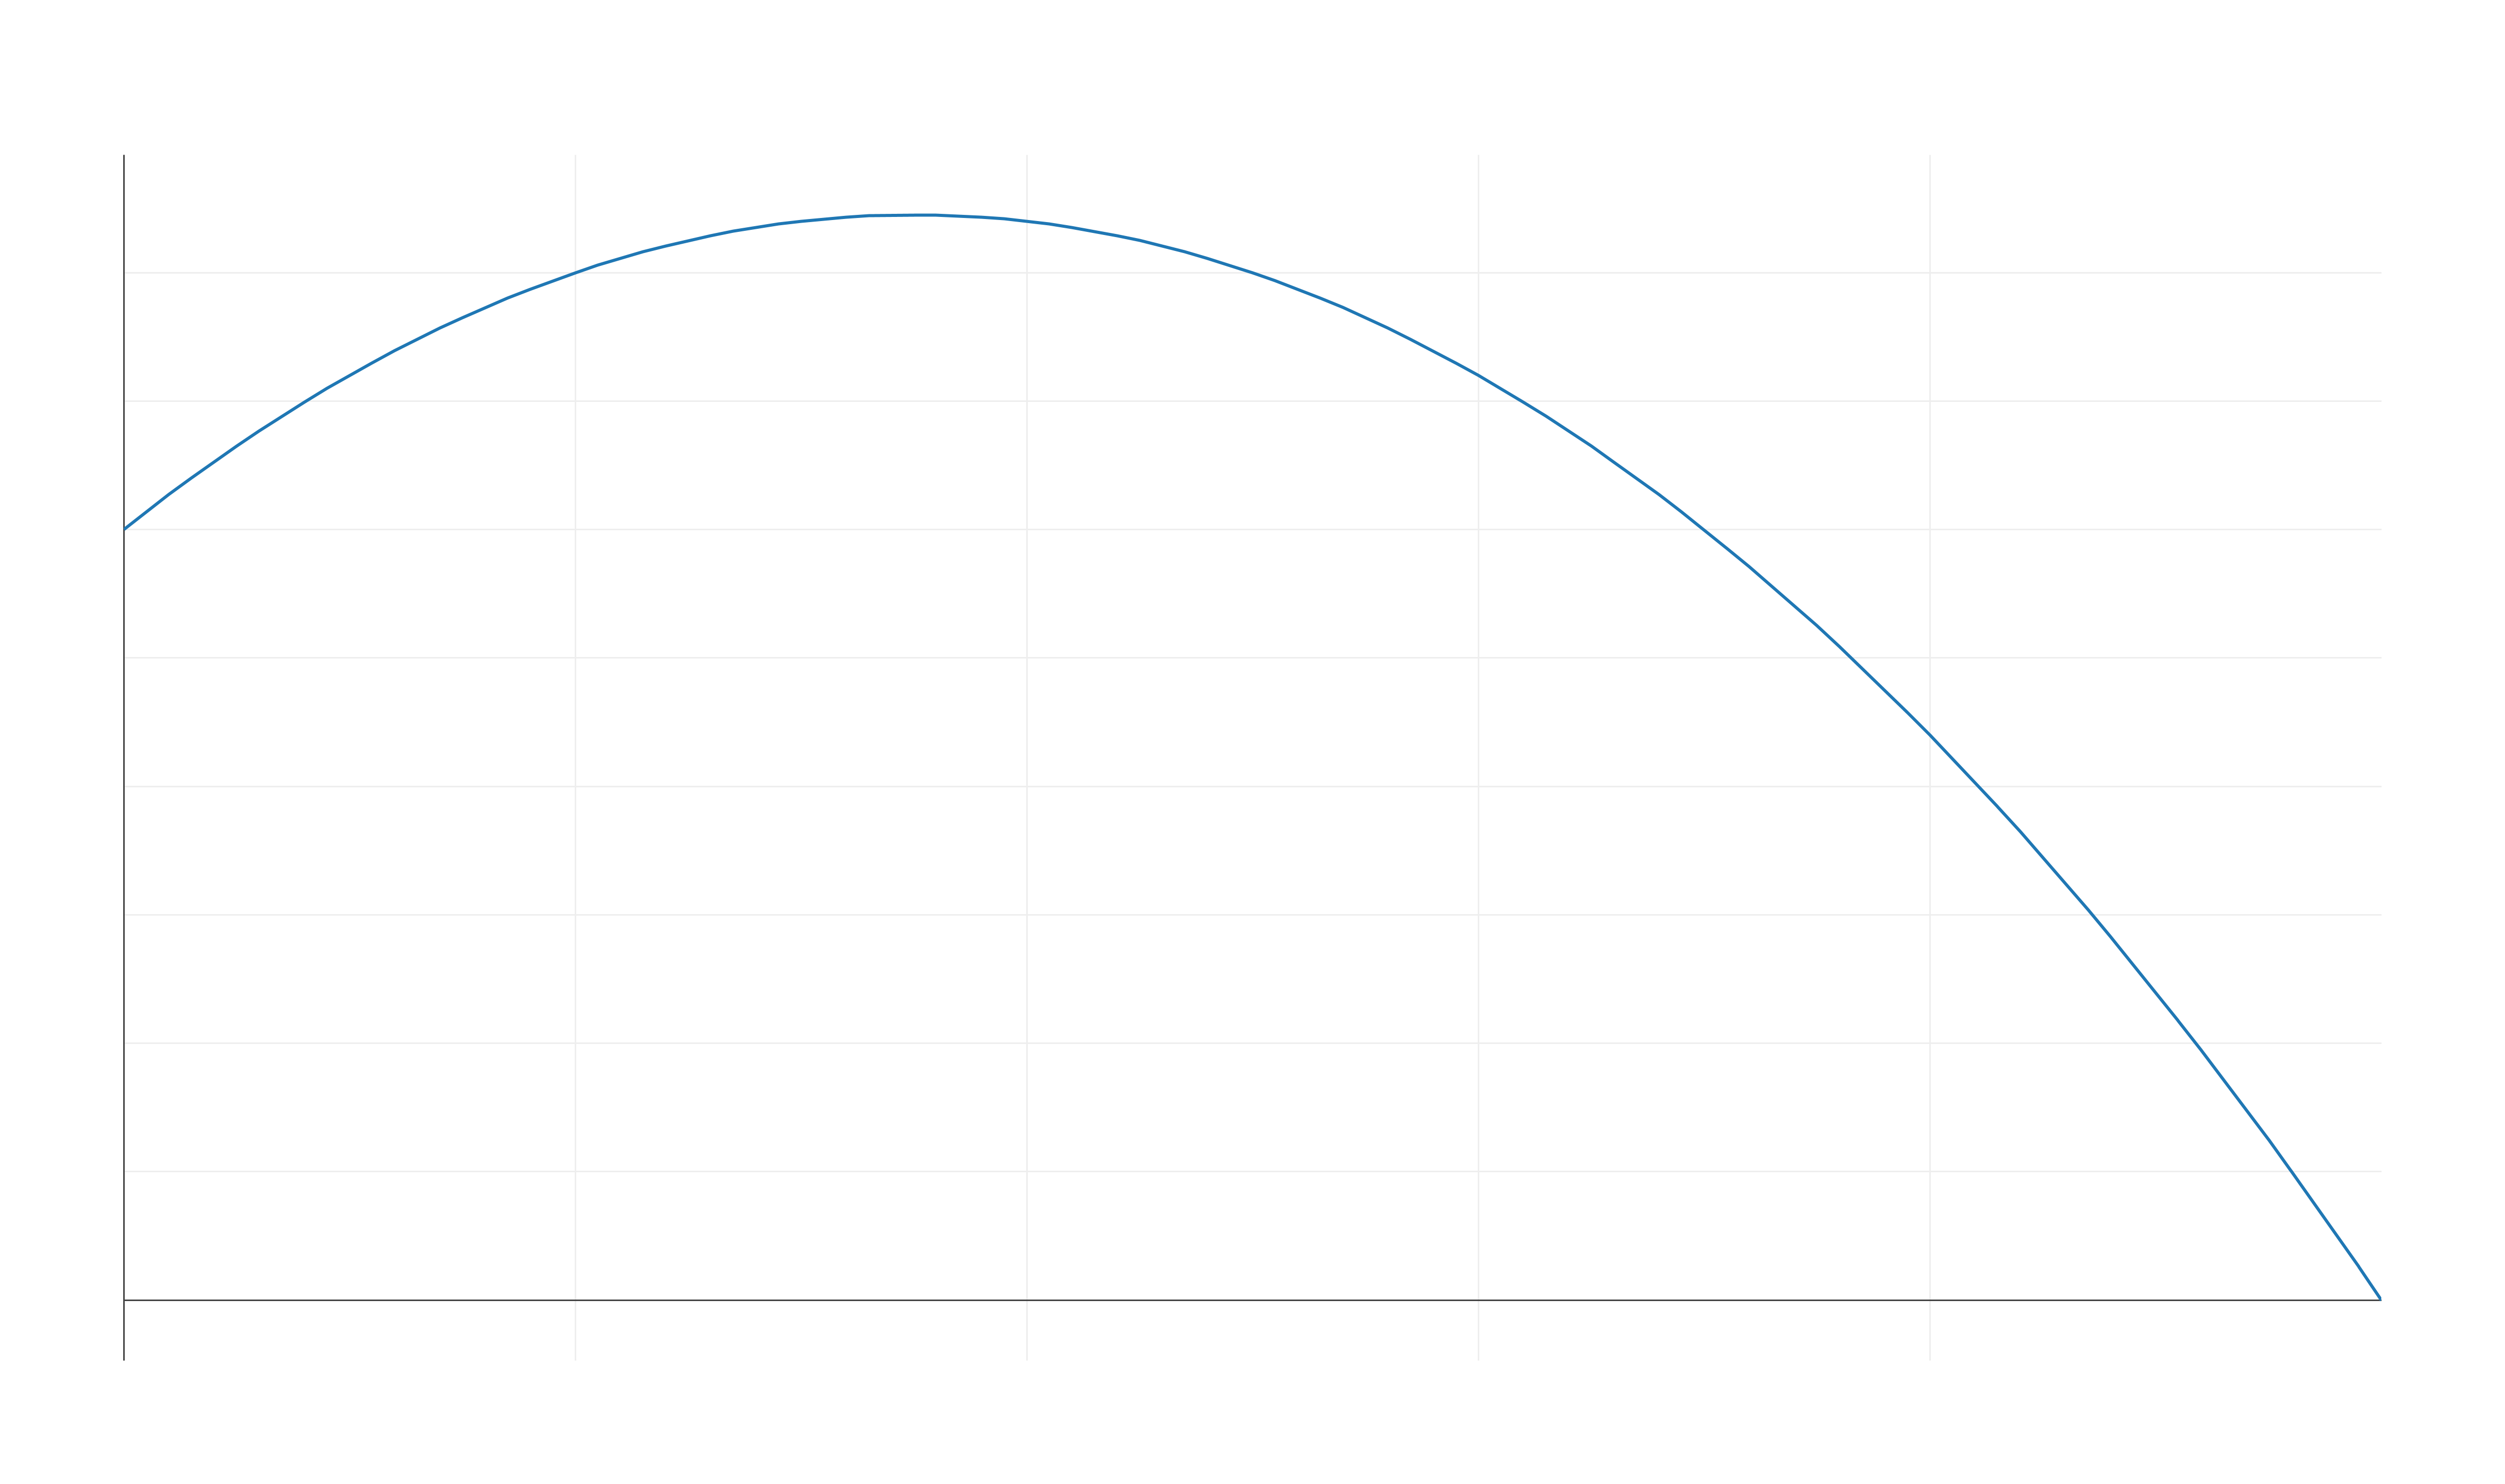
\includegraphics[scale=0.18]{resources/plot.png}
				\end{center}
			\end{block}
		\end{frame}

	\subsection{Regression Analysis}
	
		\begin{frame}
			\frametitle{Regression analysis result}
			\[
				f(x) = 400 \cdot \left[ -m \cdot \omega \cdot x^2 + (m \cdot \omega \cdot T - M_0) \cdot x + M_0 \cdot T \right]
			\]
			\[
				x_\text{max} = \frac{T}{2} - \frac{M_0}{2 \cdot m \cdot \omega}
			\]
			\[
				f_\text{max} = f(x_\text{max}) = f \left(\frac{T}{2} - \frac{M_0}{2 \cdot m \cdot \omega} \right)
			\]
			where:
			\begin{itemize}
				\item
					$m$ is the increase in contribution productivity ($0.01$)
				\item
					$T$ is the number of periods
				\item
					$x$ is the stage when players switch to contributing.
					The number before the decimal point defines a period.
					The number after the decimal point defines an investment in that period.
			\end{itemize}
		\end{frame}

		\begin{frame}
			\frametitle{In our specific case}
			\[
				f(x) = -0.1 x^2 + 0.7 x + 3
			\]
			\[
				x_{\text{optimal}} = 3.5
			\]
			
			which indicates investment until the $4_\text{th}$ period and in that period investment of $5$
			
			\[
				f_{\text{optimal}} = f(x_{\text{optimal}}) = 169
			\]
			
			which implies the payoff of $169$.
		\end{frame}
